\clearpage
\begingroup
\setlength{\parskip}{8pt}
\section{绘制时选用的资源}\label{sec:bind-api}
着色器和贴图都创建好后，还要告诉显卡本次画墙用哪一套程序、哪几个顶点、哪张贴图。这个动作叫绑定\termenglish{binding}。下例中 \code{cmd} 是正在记录主绘制的命令缓冲区。\code{graphics} 代表 \code{VK\_PIPELINE\_BIND\_POINT\_GRAPHICS}，表示这些资源用于图形绘制。

\codewhere{参数示例}{Redflag/src/Platform/Vulkan/VulkanDraw.cpp}{VulkanDraw::DrawIndexed}
\begin{lstlisting}
vkCmdBindPipeline(cmd, graphics, wallPipeline);

VkBuffer buffers[] = {wallVertices};
VkDeviceSize byteOffsets[] = {0};
(*@\rhicomment{// 两份缓冲各有自己的字节起点，这里都从开头读。}@*)
vkCmdBindVertexBuffers(cmd, 0, 1, buffers, byteOffsets);
vkCmdBindIndexBuffer(cmd, wallIndices, 0, VK_INDEX_TYPE_UINT32);
\end{lstlisting}

第一行选用刚创建的墙面管线 \code{wallPipeline}。接下来的顶点绑定从第 \code{0} 个顶点输入位置开始，这次只绑定 \code{1} 个缓冲区。\code{buffers} 给出缓冲区，\code{byteOffsets} 给出每个缓冲区从哪个字节读起。这里的位置和贴图坐标都保存在同一个顶点缓冲区里，所以两个数组各有一项。

最后一行指定索引缓冲区 \code{wallIndices}，从第 0 字节读起。类型 \code{VK\_INDEX\_TYPE\_UINT32} 表示每四个字节读成一个无符号编号。至于实际读几个编号，要到下一页发出绘制命令时才指定。

\codewhere{分组方案伪代码 · 对照}{Redflag/src/Platform/Vulkan/VulkanDraw.cpp}{VulkanDraw::DrawIndexed}
\begin{lstlisting}
(*@\rhicomment{// 这里演示按用途分三组；现行三组分别供底色、法线和透明贴图使用。}@*)
VkDescriptorSet sets[] = {frameSet, materialSet, objectSet};
vkCmdBindDescriptorSets(cmd, graphics, layout,
                        0, 3, sets, 0, nullptr);
\end{lstlisting}

描述符集\termenglish{descriptor set} 把一组着色器要用的资源列在一起。例如，\code{materialSet} 告诉着色器砖墙贴图在哪，以及怎样采样它。\code{layout} 是与管线相配的布局，规定各组装什么。\code{0, 3, sets} 表示从第 0 组起依次绑定数组中的三组，分别供本帧、材质和当前物体使用。

这个例子给每份数据预先选好了读取范围，绑定时无需额外移动起点，因此最后两个参数是 \code{0, nullptr}。如果改用动态偏移，前者填偏移量的个数，后者指向保存这些字节数的数组。

\noindent\begin{minipage}[c]{.40\linewidth}
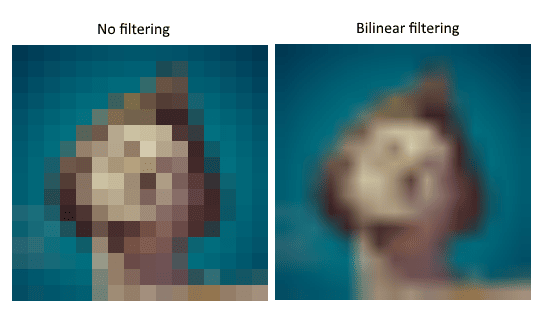
\includegraphics[width=\linewidth]{figures/khronos-filtering.png}
\end{minipage}\hfill
\begin{minipage}[c]{.56\linewidth}
{\sffamily\bfseries\color{Teal}同一张贴图的两种读法}\par\smallskip
{\small 左边只取最近的纹素，放大后能看见方格。右边按距离混合周围四个纹素，轮廓的颜色就平滑过渡。这条取色规则保存在采样器里，换规则时仍可沿用纹理里的像素。}\par\smallskip
{\footnotesize\color{Muted}\href{https://docs.vulkan.org/tutorial/latest/06_Texture_mapping/01_Image_view_and_sampler.html}{Khronos Vulkan Tutorial，Samplers 原图}。A. Overvoorde 与 The Khronos Group，\href{https://creativecommons.org/licenses/by/4.0/}{CC BY 4.0}。}
\end{minipage}
\readings{\refitem{https://docs.vulkan.org/refpages/latest/refpages/source/vkCmdBindPipeline.html}{Khronos · 绑定管线}\quad
\refitem{https://docs.vulkan.org/refpages/latest/refpages/source/vkCmdBindVertexBuffers.html}{顶点}\quad
\refitem{https://docs.vulkan.org/refpages/latest/refpages/source/vkCmdBindIndexBuffer.html}{索引}\quad
\refitem{https://docs.vulkan.org/refpages/latest/refpages/source/vkCmdBindDescriptorSets.html}{描述符集}}

\endgroup

\clearpage
\section{六个索引与一次提交}\label{sec:draw-api}
把墙的四个角依次编号为 0、1、2、3，索引缓冲区中存入
\code{0, 1, 2, 2, 3, 0}。管线按每三个索引组成一个三角形。下面这一行就是此次绘制调用\termenglish{draw call}，它把画两个三角形的请求记录到 \code{cmd} 中。

\codewhere{参数示例}{Redflag/src/Platform/Vulkan/VulkanDraw.cpp}{VulkanDraw::DrawIndexed}
\begin{lstlisting}
(*@\rhicomment{// 读六个索引，画一个实例，索引与顶点都从零开始。}@*)
vkCmdDrawIndexed(cmd, 6, 1, 0, 0, 0);
\end{lstlisting}

\noindent\begin{tabularx}{\linewidth}{@{}l@{\hspace{1.1em}}l@{\hspace{1em}}X@{}}
\toprule
参数 & 本例传值 & 画这面墙时怎样理解\\\midrule
\code{commandBuffer} & \code{cmd} & 将绘制记到这份命令缓冲区。\\
\code{indexCount} & 6 & 读六个索引，构成两个三角形。\\
\code{instanceCount} & 1 & 画一份墙面网格。\\
\code{firstIndex} & 0 & 从索引序列第 0 项开始读，单位是索引。\\
\code{vertexOffset} & 0 & 给读出的每个顶点编号加 0，再取对应顶点。\\
\code{firstInstance} & 0 & 这一批从实例编号 0 开始。\\
\bottomrule
\end{tabularx}

例如只画第二个三角形，改为 \code{vkCmdDrawIndexed(cmd, 3, 1, 3, 0, 0)}。从第 3 项开始读三个索引，正好是 \code{2, 3, 0}。这里传的是 3；换算成这组 32 位索引的字节位置才是 12。绘制时不用改动原来的索引缓冲区。

\subsection{录制完成后交给图形队列}
\codewhere{提交方案伪代码 · 现有入口}{Redflag/src/Platform/Vulkan/VulkanContext.cpp}{VulkanContext::SwapBuffers}
\begin{lstlisting}
(*@\rhicomment{// 本例的围栏 finished 通知 CPU 这一批命令已经完成。}@*)
vkQueueSubmit2(graphicsQueue, 1, &submit, finished);
\end{lstlisting}

\code{graphicsQueue} 是用来执行这批绘制的图形队列\termenglish{graphics queue}。\code{1} 表示提交一份说明，\code{\&submit} 指向这份说明。本例在其中列入已经结束录制的 \code{cmd}。\code{finished} 是这次提交使用的围栏\termenglish{fence}，提交前处于未完成状态。函数返回成功表示工作已经交给队列。等围栏收到完成信号，CPU 才知道这次提交中的复制和绘制都已经执行完。

这里画到离屏图像，因此可以单独等这只围栏。实际窗口还要等待取得窗口图像，并通知窗口可以显示。当多帧连续绘制时，项目拟用提交编号跟踪资源的回收，见第~\pageref{sec:recycle}~页。
\readings{\refitem{https://docs.vulkan.org/refpages/latest/refpages/source/vkCmdDrawIndexed.html}{Khronos · 索引绘制}\quad
\refitem{https://docs.vulkan.org/refpages/latest/refpages/source/vkQueueSubmit2.html}{队列提交}\quad
\refitem{https://docs.vulkan.org/refpages/latest/refpages/source/VkSubmitInfo2.html}{提交内容}}
